\section{Empirical evaluation}\label{sec:experiments}

In the previous section we showed that our proposed estimator has a number of desirable theoretical properties.
Next we demonstrate its practical performance.
First, we present a synthetic experiment investigating the behaviour of RAM-MC in controlled settings where all distributions and divergences are known.
Second, we investigate the use of RAM-MC in a more realistic setting to estimate a divergence between the aggregate posterior $Q_Z$ and prior $P_Z$ in pretrained autoencoder models. 
For experimental details not included in the main text,
see Appendix \ref{appendix:empirical-evaluation-details}\footnote{
A python notebook to reproduce all experiments is available at \url{https://github.com/google-research/google-research/tree/master/f_divergence_estimation_ram_mc}.}.


\subsection{Synthetic experiments}\label{section:synth-exps}
\textbf{The data model.}
Our goal in this subsection is to test the behaviour of the RAM-MC estimator for various $d=\dim(\mathcal{Z})$ and $f$-divergences.
We choose a setting in which $Q^{\lambda}_Z$ parametrized by a scalar $\lambda$ and $P_Z$ are both $d$-variate normal distributions for $d\in\{1, 4, 16\}$.
We use RAM-MC to estimate $D_f(Q^\lambda_Z, P_Z)$, which can be computed analytically for the KL, $\chi^2$, and squared Hellinger divergences in this setting (see Appendix \ref{appendix:toy-exps}).
Namely, we take ${P_Z}$ and ${Q_X}$ to be standard normal distributions over $\Z=\R^d$ and $\X=\R^{20}$ respectively,
and $\smash{Z\sim Q^\lambda_{Z|X}}$ be a linear transform of $X$ plus a fixed isotropic Gaussian noise, with the linear function parameterized by $\lambda$.
By varying $\lambda$ we can interpolate between different values for $D_f(Q_Z^\lambda \| P_Z)$.

\textbf{The estimators.}
In Figure \ref{fig:synthetic-exps} we show the behaviour of RAM-MC with $N\,{\in}\,\{1, 500\}$ and $M{=}128$ compared to the ground truth as $\lambda$ is varied. 
The columns of Figure~\ref{fig:synthetic-exps} correspond to different dimensions $d\,{\in}\,\{1, 4, 16\}$, and rows to the $\KL$, $\chi^2$ and $\mathrm{H}^2$ divergences, respectively. 
We also include two baseline methods.
First, a plug-in method based on kernel density estimation \cite{moon14ensemble}.
Second, and only for the KL case, the M1 method of~\cite{nguyen10ratio} based on density ratio estimation.

\textbf{The experiment.}
To produce each plot, the following was performed 10 times, with the mean result giving the bold lines and standard deviation giving the error bars.
First, $N$ points $\XN$ were drawn from $Q_X$. 
Then $M{=}128$ points $\ZM$ were drawn from $\hat{Q}_Z^N$ and RAM-MC \eqref{eq:our-mc-estimate} was evaluated. 
For the plug-in estimator, the densities $\hat{q}(z)$ and $\hat{p}(z)$ were estimated by kernel density estimation with 500 samples from $Q_Z$ and $P_Z$ respectively using the default settings of the Python library {\texttt{scipy.stats.gaussian\_kde}}.
The divergence was then estimated via MC-sampling using $128$ samples from $Q_Z$ and the surrogate densities.
The M1~estimator involves solving a convex linear program in $N$ variables to maximize a lower bound on the true divergence, see \cite{nguyen10ratio} for more details.
Although the M1~estimator can in principle be used for arbitrary $f$-divergences, its implementation requires hand-crafted derivations that are supplied only for the $\KL$ in \cite{nguyen10ratio}, which are the ones we use.

\textbf{Discussion.}
The results of this experiment empirically support Proposition \ref{prop:upper-bound} and Theorems \ref{thm:fast-KL-rate}, \ref{thm:convergence-rate-general}, and~\ref{thm:mc-variance}:
(i) in expectation, RAM-MC upper bounds the true divergence; (ii) by increasing $N$ from 1 to 500 we clearly decrease both the bias and the variance of RAM-MC.
When the dimension $d$ increases, the bias for fixed $N$ also increases.
This is consistent with the theory in that, although the rates are independent of $d$, the constants are not.
We note that by side-stepping the issue of density estimation, RAM-MC performs favourably compared to the plug-in and M1 estimators, more so in higher dimensions ($d=16$).
In particular, the shape of the RAM-MC curve follows that of the truth for each divergence, while that of the plug-in estimator does not for larger dimensions.
In some cases the plug-in estimator can even take negative values because of the large variance.


\begin{figure}
\begin{center}
\begin{tikzpicture}
\node[anchor=south west,inner sep=0] at (0,0) {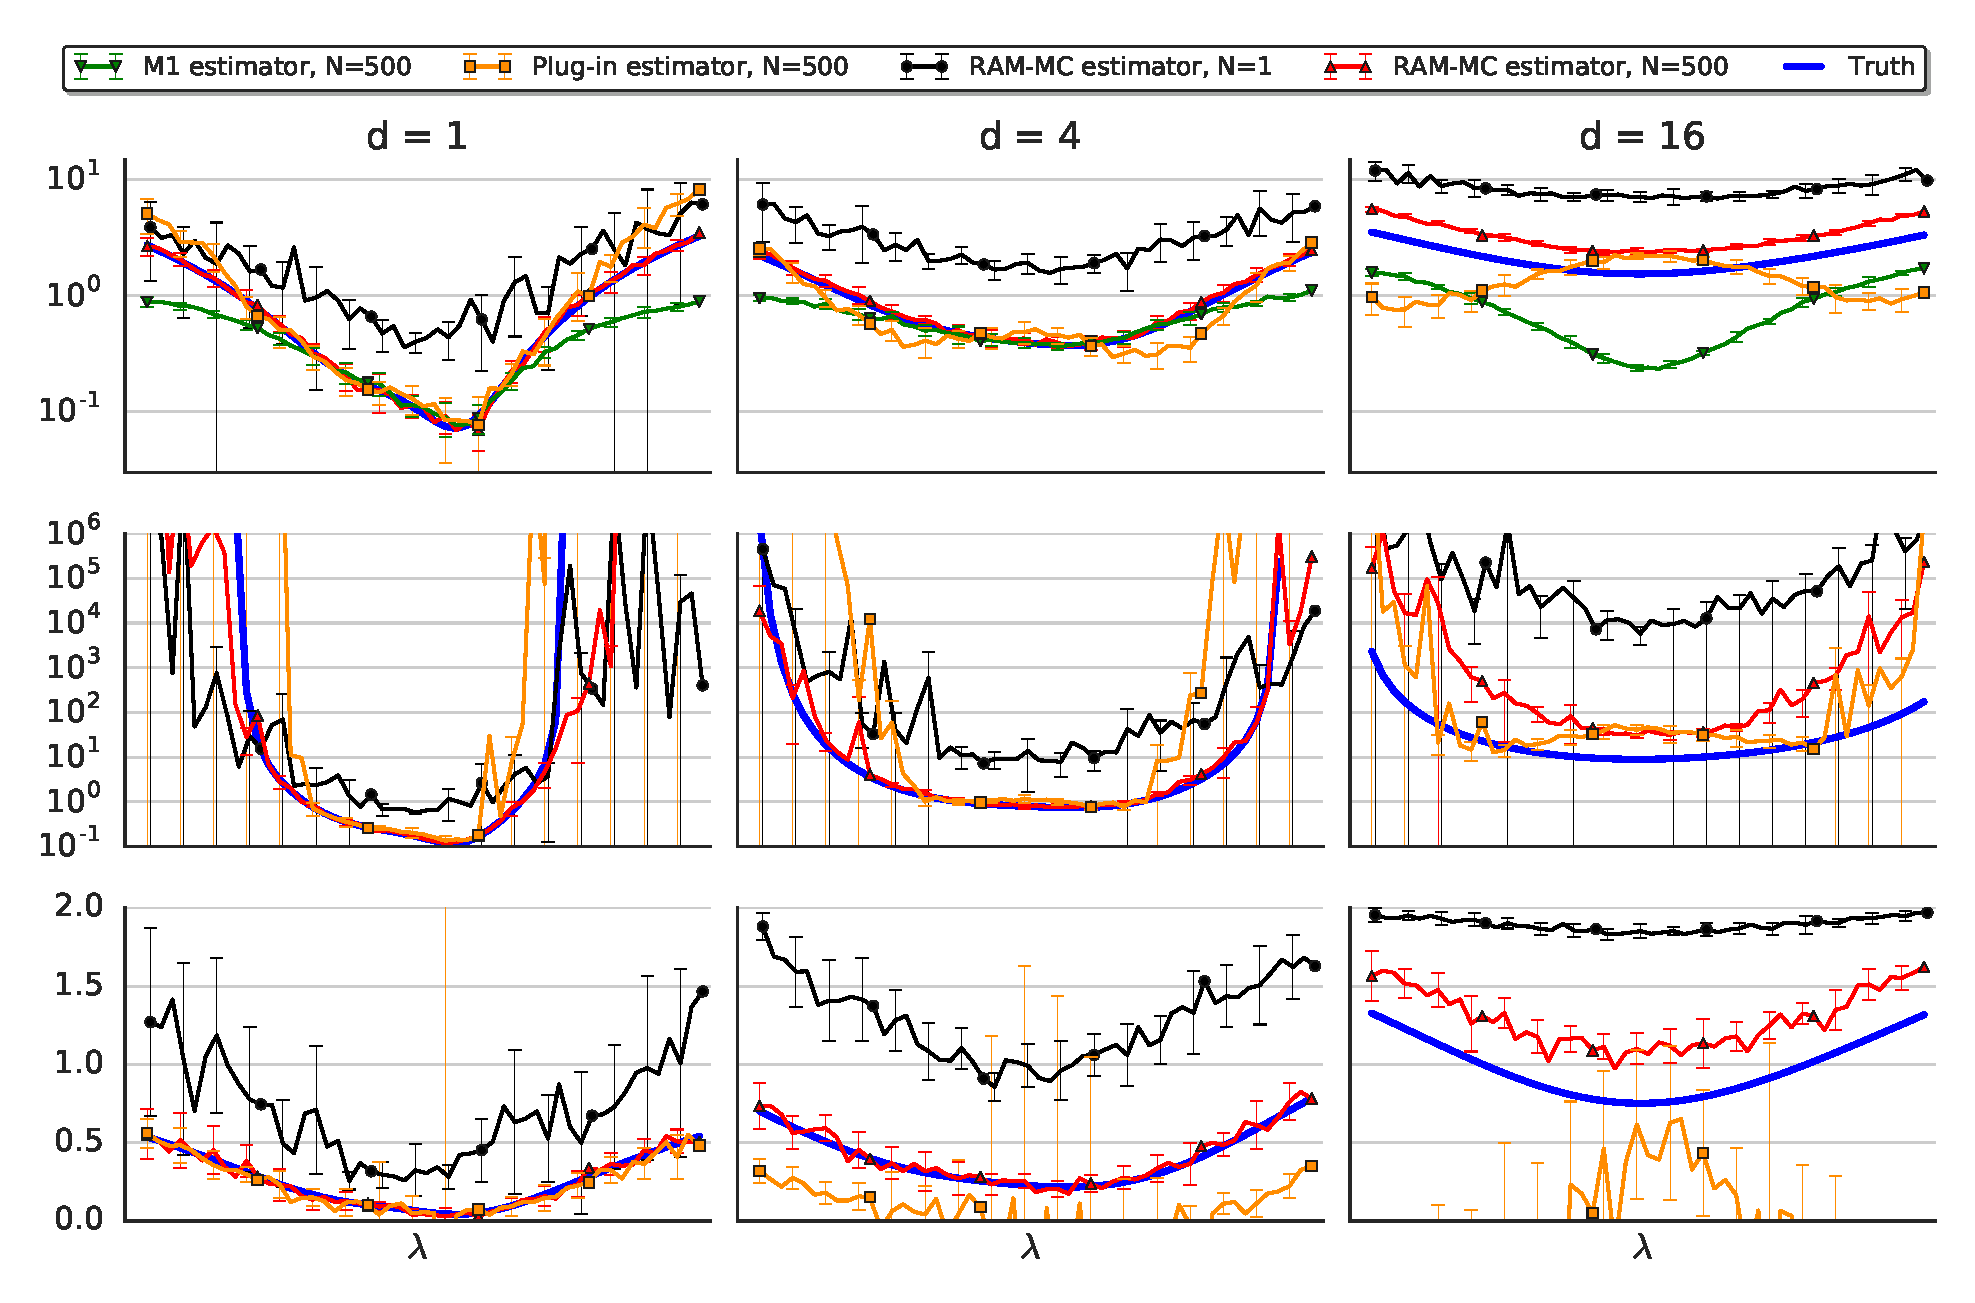
\includegraphics[width=0.97\textwidth, height=0.615\textwidth]{pics/NeurIPS_toy_exps_plot.pdf}};
\node[rotate=0] at (0, 1.7) {$\mathrm{H}^2$};
\node[rotate=0] at (0, 4.2) {$\chi^2$};
\node[rotate=0] at (0, 6.7) {$\mathrm{KL}$};
\end{tikzpicture}
\end{center}
\caption{\label{fig:synthetic-exps}
(Section~\ref{section:synth-exps})
Estimating $D_f\bigl(\mathcal{N}(\mu_\lambda, \Sigma_\lambda),\, \mathcal{N}(0, I_d)\bigr)$ for various $f$, $d$, and parameters $\mu_\lambda$ and $\Sigma_\lambda$ indexed by $\lambda\in \R$.
Horizontal axis correspond to $\lambda\in[-2, 2]$,
columns to $d\in\{1, 4, 16\}$ and
rows to KL, $\chi^2$, and $\mathrm{H}^2$ divergences respectively.
{\bf \textcolor{blue}{Blue}} are true divergences, 
{\bf black} and {\bf \textcolor{red}{red}} are RAM-MC estimators~\eqref{eq:our-mc-estimate} for $N\in\{1, 500\}$ respectively,
{\bf \textcolor{darkgreen}{green}} are M1 estimator of~\citep{nguyen10ratio} and {\bf \textcolor{orange}{orange}} are plug-in estimates based on Gaussian kernel density estimation \citep{moon14ensemble}.
$N=500$ and $M=128$ in all the plots if not specified otherwise.
Error bars depict one standard deviation over 10 experiments.
}
\end{figure}

\subsection{Real-data experiments}
\label{sec:exp_wae}
\textbf{The data model.}
To investigate the behaviour of RAM-MC in a more realistic setting, we consider Variational Autoencoders (VAEs) and Wasserstein Autoencoders (WAEs) \cite{kingma2013auto, tolstikhin2017wasserstein}.
Both models involve learning an \emph{encoder} $\smash{Q^\theta_{Z|X}}$ with parameter $\theta$ mapping from high dimensional data to a lower dimensional latent space and decoder mapping in the reverse direction.
A prior distribution ${P_Z}$ is specified, and the 
optimization objectives of both models are of the form ``reconstruction + distribution matching penalty''.
The penalty of the VAE was shown by \cite{hoffman2016elbo} to be equivalent to $\smash{\KL(Q^\theta_Z \| P_Z) + I(X,Z)}$ where $I(X,Z)$ is the mutual information of a sample and its encoding.
The WAE penalty is ${D(Q^\theta_Z \| P_Z)}$ for any divergence $D$ that can practically be estimated.
Following \cite{tolstikhin2017wasserstein}, we trained models using the Maximum Mean Discrepency (MMD), a kernel-based distance on distributions, and a divergence estimated using a GAN-style classifier leading to WAE-MMD and WAE-GAN respectively \cite{gretton2012kernel, goodfellow2014generative}.
% Both of them can be estimated from samples.
For more information about VAE and WAE, see Appendix \ref{appendix:intro-vae-wae}.

\textbf{The experiment.}
We consider models pre-trained on the \emph{CelebA} dataset \cite{liu2015faceattributes}, 
and use them to evaluate the RAM-MC estimator as follows.
We take the test dataset as the ground-truth $Q_X$, and embed it into the latent space via the trained encoder.
As a result, we obtain a ${\sim}{20}\text{k}$-component Gaussian mixture for $Q_Z$, the \emph{empirical aggregate posterior}. 
Since $Q_Z$ is a finite---not continuous--- mixture, the true $D_f(Q_Z\|P_Z)$ can be estimated using a large number of MC samples (we used $10^4$).
Note that this is very costly and involves evaluating $2\cdot 10^4$ Gaussian densities for each of the $10^4$ MC points.
We repeated this evaluation 10 times and report means and standard deviations.
RAM-MC is evaluated using $N \in \{2^0, 2^1,\ldots, 2^{14}\}$ and $M \in \{10, 10^3\}$.
For each combination $(N,M)$, RAM-MC was computed 50 times with the means plotted as bold lines and standard deviations as error bars.
In Figure~\ref{fig:real-exps} we show the result of performing this for the KL divergence on six different models.
For each dimension $d\in\{32, 64, 128\}$, we chose two models from the classes (VAE, WAE-MMD, WAE-GAN). 
See Appendix~\ref{appendix:real-data-experiments-additional} for further details and similar plots for the $H^2$-divergence.

\textbf{Discussion.}
The results are encouraging. 
In all cases RAM-MC achieves a reasonable accuracy with $N$ relatively small, even for the bottom right model where the true KL divergence ($\approx 1910$) is very big.
We see evidence supporting Theorem~\ref{thm:mc-variance}, which says that the variance of RAM-MC is mostly determined by the smaller of $\psi(N)$ and $M$:
when $N$ is small, the variance of RAM-MC does not change significantly with $M$, 
however when $N$ is large, increasing $M$ significantly reduces the variance. 
Also we found there to be two general modes of behaviour of RAM-MC across the six trained models we considered. 
In the bottom row of Figure~\ref{fig:real-exps} we see that the decrease in bias with $N$ is very obvious, supporting Proposition~\ref{prop:upper-bound} and Theorems \ref{thm:fast-KL-rate} and \ref{thm:convergence-rate-general}.
In contrast, in the top row it is less obvious, because the comparatively larger variance for $M{=}10$ dominates reductions in the bias.
Even in this case, both the bias and variance of RAM-MC with $M{=}1000$ become negligible for large $N$.
Importantly, the behaviour of RAM-MC does not degrade in higher dimensions.


The baseline estimators (plug-in \cite{moon14ensemble} and M1~\cite{nguyen10ratio}) perform so poorly that we decided not to include them in the plots (doing so would distort the $y$-axis scale).
In contrast, even with a relatively modest $N{=}2^8$ and $M{=}1000$ samples, RAM-MC behaves reasonably well in all cases.

\begin{figure}
\begin{center}
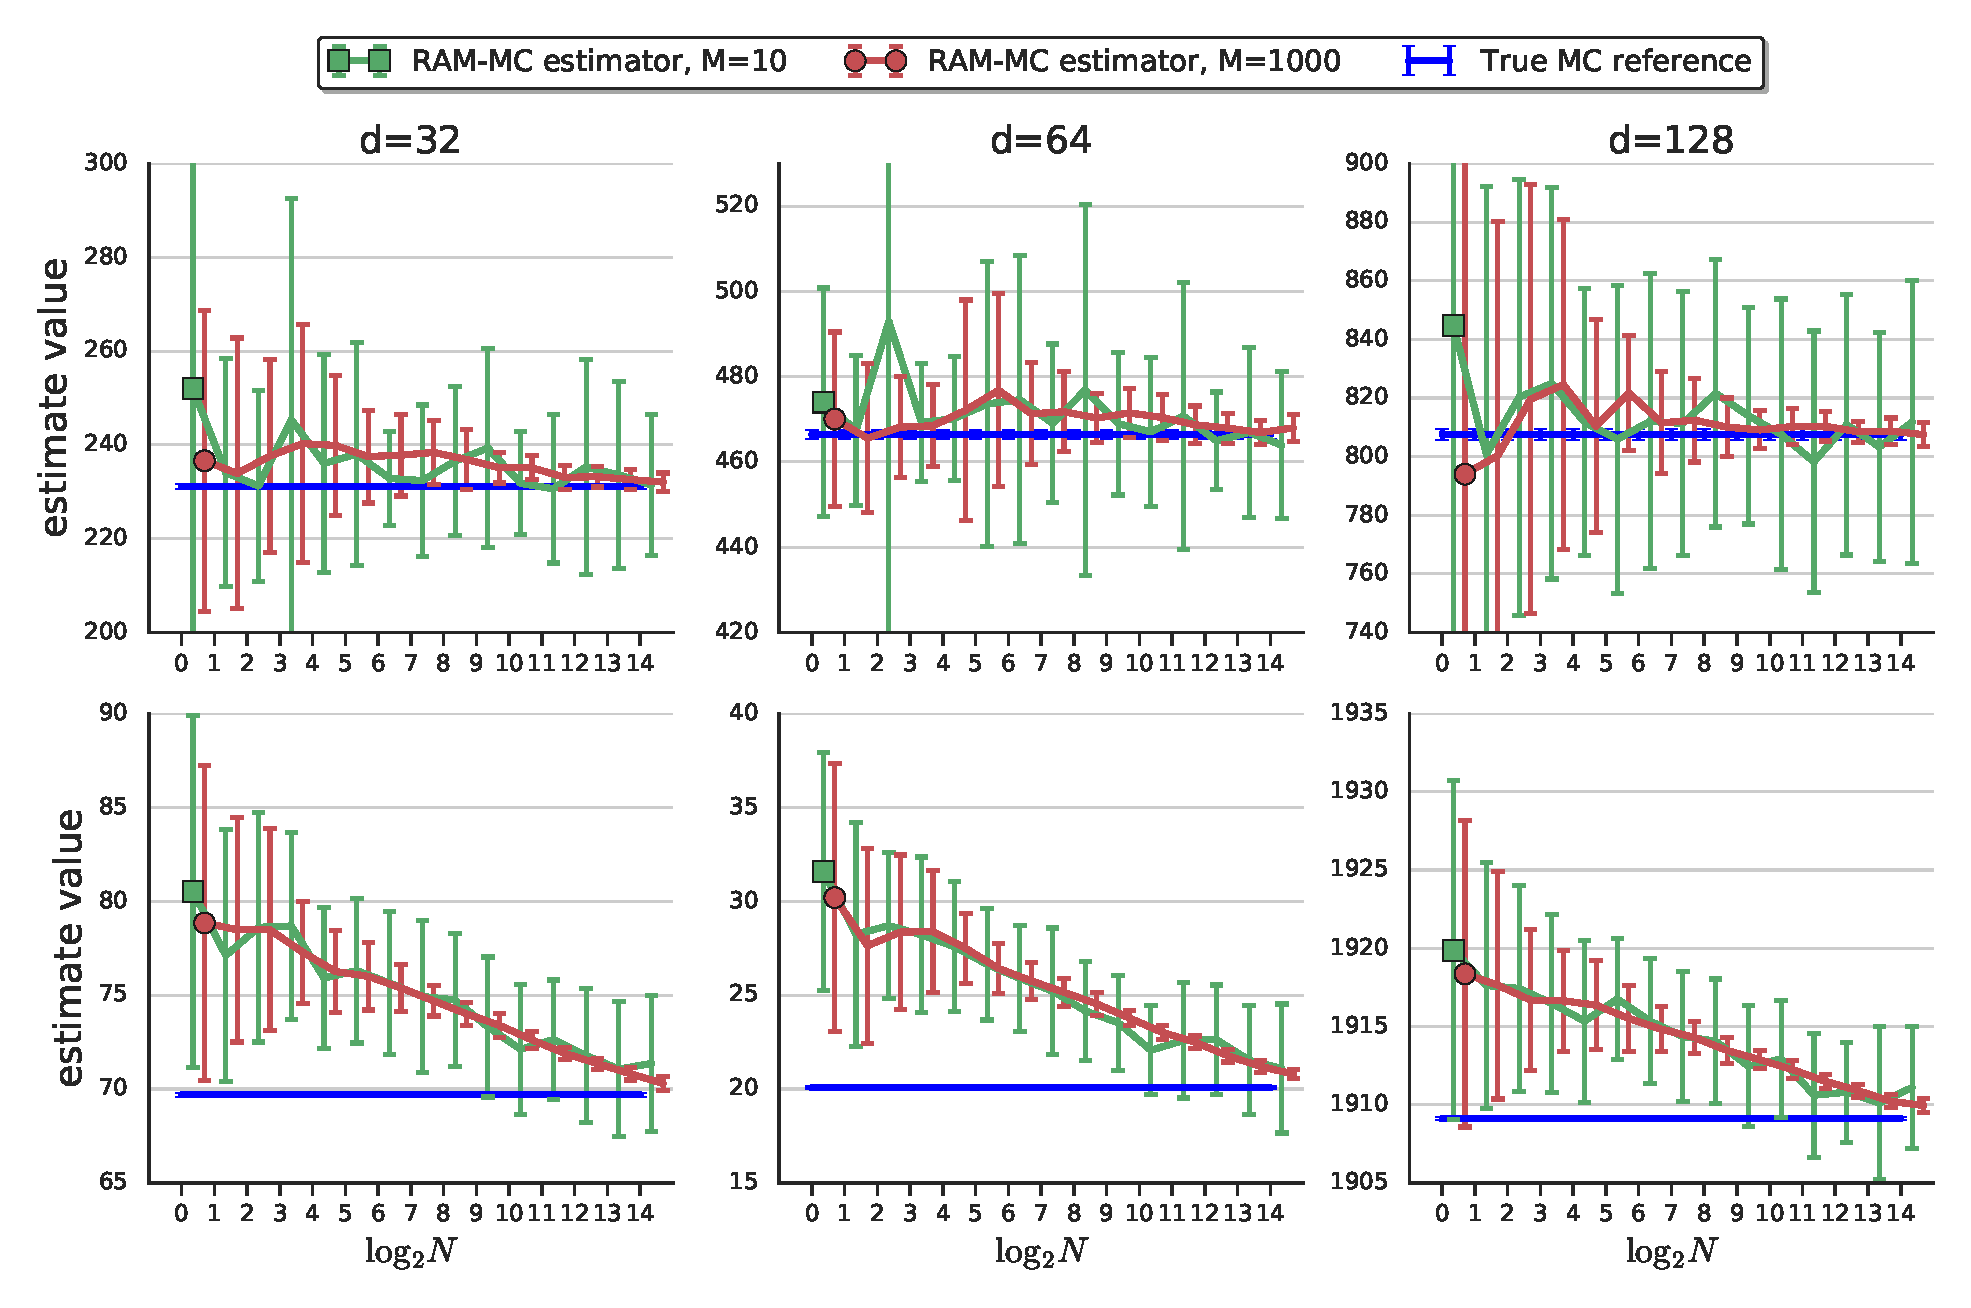
\includegraphics[width=1.\textwidth, height=0.615\textwidth]{pics/NeurIPS_wae_exps_plot.pdf}
\end{center}
\caption{\label{fig:real-exps}
(Section~\ref{sec:exp_wae}) Estimates of $KL(Q_Z^\theta \| P_Z)$ for pretrained autoencoder models with RAM-MC as a function of $N$ for $M{=}10$ ({\bf \textcolor{green!65!blue}{green}}) and $M{=}1000$ ({\bf \textcolor{red}{red}}) compared to an accurate MC estimate of the ground truth ({\bf\textcolor{blue}{blue}}).
Lines and error bars represent means and standard deviations over 50 trials.
}
\end{figure}